\section{The Intel 486}

\begin{wrapfigure}[5]{r}{0.25\textwidth}
\centering

\includegraphics[width=.25\textwidth]{drawings/intel_logo.pdf}
\end{wrapfigure}

Announced in 1989, the 80486 was a performance evolution which addressed all bottlenecks of the 80386. However its price tag of \$950 (\$1,920 in 2018) kept it away from most consumers. By 1993 it was finally becoming affordable (\$500) and would become \doom{}'s recommended CPU.\\
\par
The design had changed significantly compared to its predecessor. The pipeline was gifted with two extra stages, extending its depth to five elements. The FPU\footnote{Floating Point Unit.} which used to be optional and somewhere on the motherboard was brought on-die. Most importantly, manufacturing improvements\footnote{Manufacturing technology improved from 1.5$\mu$ to 1.0$\mu$ allowing five times more transistors on die.} allowed the 486 a more elaborate design to finally feature an integrated L1 cache.\\
\par
\fq{The 386 actually had a small cache that eventually got exited because it didn't have enough performance for the size of the cache that we could put on board the chip, and the problem was if you made the chip bigger, it literally wouldn't fit inside the lithography machine's field of view, to flash on the chip.}{Gene Hill - Intel 386 Microprocessor Design and Development}\\
\par

\drawing{486_arch}{Intel 486 architecture}
\par
Like with the 386, Intel marketed its new CPU in two flavors. A DX version which was the pure technology and an SX version with an unavailable FPU. A decades diehard myth is that the DX/SX distinction was a marketing stunt from Intel to sell chips coming out of the factory with malfunctioning parts due to manufacturing problems. It was in fact an intentional commercial operation\footnote{Source: "Lies, Damn Lies, and Wikipedia" by Michal Necasek ; The timeline did not make sense since "The 486DX started shipping in volume in late 1989. The 486SX was only introduced in mid-1991. In the first 18 months or so when yield problems would have been the worst, there was no SX.".} to provide a discounted (50\%) price and an opportunity to sell i487 FPU co-processors.\footnote{Amusingly, the i487 FPU upgrade was a full blown 486DX which disabled the 486SX completely!}.\\
\par
If in retrospect the 486 was Intel's 1994 champion and an unquestionable powerhouse (both in terms of performances and sales\footnote{As of late 2015, the 486 was still manufactured and used inside network routers.}), it had to sustain a period of uncertainty. Like the 386 had to face its brother (the i960), the i486 also had to a competitor from the same company. The competing brother name was "Intel 860".\\
\par
\fq{

\begin{wrapfigure}[11]{r}{0.55\textwidth}
\centering
\scaledimage{0.55}{i860.png}
\end{wrapfigure}

...We now had two very powerful chips that we were introducing at just about the same time: the 486, largely based on CISC technology and compatible with all the pc software, and the i860, based on RISC technology, which was very fast but compatible with nothing. We didn't know what to do. So we introduced both, figuring we'd let the marketplace decide. However, things were not that simple. Supporting a microprocessor architecture with all the necessary computer-related products --- software, sales, and technical support --- takes enormous resources. Even a company like Intel had to strain to do an adequate job with just one architecture. And now we had two different and competing efforts, each demanding more and more internal resources. Development projects have a tendency to want to grow like the proverbial mustard seed. The fight for resources and for marketing attention (for example, when meeting with the customer, which processor should we highlight) led to internal debates that were fierce enough to tear apart our microprocessor organization. Meanwhile, our equivocation caused our customers to wonder what Intel really stood for, the 486 or i860?}{Andy Grove, "Only the paranoid survive".}





On paper, the i860 was impressive and a serious competitor. Relying on an heavily pipelined super-scalar architecture crushing VLIWs\footnote{Very Long Instruction Word.}. It had three units, X, Y, and Z allowing parallel processing which when efficiently used could outperform the Intel 486.\\
\par
But where later CPUs such as the Pentium chose to hide the chip complexity by automatically executing instruction in parallel when possible, the i860 architecture mandated direct manipulation to its parallel pipelines. The chip did nothing behind the scenes and relied on compiler writers to sequence instructions appropriately.\\
\par
Unfortunately, compiler technology was not there yet. Without Intel's full backing to generate the precious tool, none of the compilers available came even remotely close to generating instructions able to exploit its super-scalar capability. The i860 was never able to reach its full potential. If only Intel had been willing to build the tools it desperately needed, the history of the i860 could have been different.\\
\par
\par
\cscaledimage{0.85}{i486DX.png}{}
\par
In figure \ref{i486DX.png}, the Intel 486 die and its 1,180,235 transistors inside a package. Around this time period, Intel's started to stamp its CPU with trademarked logo in an attempt to distance itself from increasingly aggressive AMD and Cyrix clones.\\
\par
\trivia{The i860 played a part in \doom{} anyway since it was used in NextDimension video processing boards.}

\par
\subsection{Pipeline improvements}
Charting the 486 MIPS performance along with the previous generation make the performance boost appear vividly. Thanks to an improved manufacturing process, top of the line 486 were able to run at 50Mhz\footnote{To reach this frequency, 486 DX 50Mhz were manufactured at 1.0$\mu$.} but frequency increase was not the main factor of improvement.\\
\par
 Looking closely at the chart, one will notice that even at equal frequency, a 486 offered more than twice the processing power of a 386.\\

\par
\begin{figure}[H]
\centering
  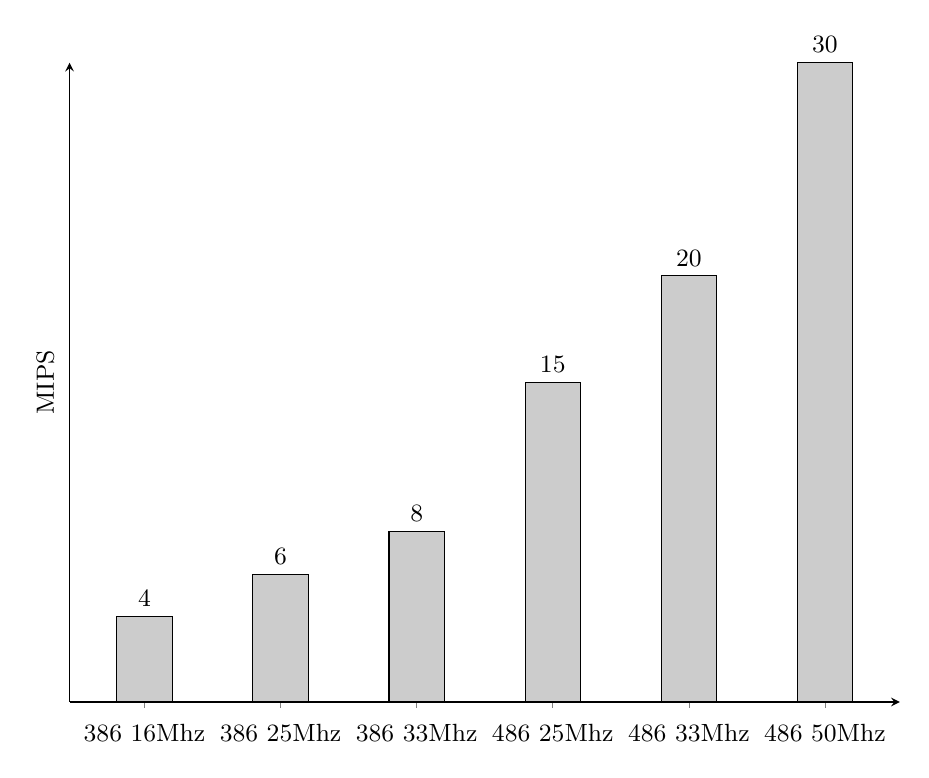
\begin{tikzpicture}[font=\small]
    \begin{axis}[
      width=1.0\textwidth,
      height=0.8\textwidth,
      ybar,
      bar width=20pt,
      ylabel={MIPS},
      ymin=0,
      ytick=\empty,
      xtick=data,
      axis x line=bottom,
      axis y line=left,
      enlarge x limits=0.11,
      symbolic x coords={386 16Mhz,386 25Mhz,386 33Mhz,486 25Mhz,486 33Mhz,486 50Mhz},
      xticklabel style={anchor=base,yshift=-\baselineskip},
      nodes near coords={\pgfmathprintnumber\pgfplotspointmeta}
    ]
      \addplot[fill=black!20,draw=black] coordinates {
        (386 16Mhz,4)
        (386 25Mhz,6)
        (386 33Mhz,8)
        (486 25Mhz,15)
        (486 33Mhz,20)
        (486 50Mhz,30)
      };
    \end{axis}
   
   \end{tikzpicture}
   \caption{Comparison\protect\footnotemark of Intel CPUs with MIPS \protect\footnotemark.}
 \end{figure}
\footnotetext{Source: "Roy Longbottom's PC Benchmark Collection: http://www.roylongbottom.org.uk/mips.htm".}

The way it achieves higher performances is through a higher average throughput. According to its documentation the 386 was a smooth three stage pipelined processor. Under ideal conditions, figure \ref{386_doc_pipeline} shows how it should have in theory been able to execute one instruction per cycle. In practice the CPU behaved as shown in figure \ref{386_real_pipeline}, twice slower than suggested.

\begin{figure}[H]
\centering
\includegraphics[width=\textwidth]{drawings/386_instruction_pipeline.pdf}
\caption{386 pipeline in theory according to Intel documentation.}
\label{386_doc_pipeline}
\end{figure}



\par
Even if the Prefetch Unit and the Execution Unit were properly fed, the Decode unit always took a minimum of two cycles to decode an instruction\footnote{The author speculates this high decode cost was the result of Intel's choice to use CISC instead of RISC.}. Since the maximum throughput of a pipeline cannot exceed the speed of its slowest stage, the Intel 386 could process at most one instructions every two cycles.\\
\par

\begin{figure}[H]
\centering
\includegraphics[width=\textwidth]{drawings/actual_386_instruction_pipeline.pdf}
\caption{386 pipeline in practice: Two cycles per instruction.}
\label{386_real_pipeline}
\end{figure}

\par
To solve this problem, Intel broke down the three stage pipeline into five (Prefetch, Decode1, Decode2, Execute, WriteBack). With all stages performing at 1 CPI\footnote{Cycle Per Instruction.}, the total throughput of the 486 was doubled (as long as the pipeline never starved).\\
\par
\begin{figure}[H]
\centering
\includegraphics[width=\textwidth]{drawings/actual_486_instruction_pipeline.pdf}
\caption{486 pipeline: One cycle per instruction.}
\end{figure}
\par





\subsection{Caching }
Modifying the pipeline and make each stage run as fast as each others was one step in the right direction. But making the pipeline deeper also made it more vulnerable to starvation. Starting from an empty pipeline, the 486 had a latency of 5 cycles compared to the 386 which had only three stages. A frequently stalling 486 would have been slower than a 386. Halting processing due to missing data or instructions was to be avoided at all cost.\\
\par
It was a difficult constraint to fulfill for physical reasons. Since 1980, RAM performances had been lagging behind CPU performances. Each year, CPU improved by 60\% while DRAM only improved by 7\%, the gap increased by 50\%/year. By 1989, DRAM access time was 10 times slower than CPU cycles.\\
\par
\vspace{2mm}
\drawing{ram_vs_cpu}{}
\par
Until the 486, a CPU requesting either instructions or datas from the DRAM always had to stall and go through its Bus Unit to talk to the motherboard memory controller. As optimized as the ISA bus protocol was, it took at the very minimum two cycles.\\
\par 
A first cycle to initialize the bus request, place the address on the address line and set the control line (Read/Write). And a wait cycle (which Intel called Wait State since while waiting on the Bus Unit, the CPU did absolutely nothing) while the device on the other side of the bus fulfilled the request.\\
\par
\drawing{cpu_chipset_bus}{386 CPU-RAM communication elements}
\par
If a device was able to answer the bus request within the first wait state cycle, the CPU was able to resume operations having reached Zero Wait state. Otherwise, additional Wait States were inserted in order to wait for the request to complete. From a performance perspective, these Wait States were a disaster. Not only because it took longer for the instruction to finish but also because it stalled all other instructions in the pipeline.\\
\par
\rawdrawing{cpu_wait_states}
\par
Two cycles bus request is the fastest a CPU can achieve. In practice, DRAM access requires several Wait State insertions.
To avoid these stales meant to avoid using the bus completely. To achieve this, Intel inserted a new component between the pipeline and the bus unit and called it a L1 (Level 1) cache. The idea was to exploit both spacial and temporal locality of a program.\\
\par
Temporal locality relies on program iterative nature. While in a loop, an instruction recently accessed is likely to be accessed again on the next iteration. Spacial locality has to do with the way program sequentially read or write arrays containing data. If a memory address is accessed, it is likely a neighboring address will also be accessed shortly after.\\
\par
By leveraging these two properties, a well designed cache located between the CPU and the Bus Unit would often already contains the data or instruction requested, making a bus request useless.\\
\par
\drawing{cpu_cache}{486 CPU-RAM communication elements}



\vspace{-20pt}
\subsection{L1 Cache}
Hopefully it is now abundantly clear the cache was the cornerstone of the entire CPU. Designing the cache to yield the highest hit rate possible and make it as fast as possible were paramount. 

\subsubsection{DRAM vs SRAM}
The first thing the cache had going on for itself is the lower latency of its RAM. If the main RAM on the SIMM slots used DRAM (Dynamic RAM) the cache was made of a different type called SRAM, able to much faster access time. DRAM typically had an access time of 200ns while SRAM was capable of 20ns, 1000\% faster. \\
\par
The difference of speed comes from the design of their elementary cells.\\
\par
 A DRAM cell hold a bit. It's simple design features one transistor and one storage capacitor which allow tight packing and high capacity. However the capacitor loses its charge over time and each time it is accessed. Every time the cell is read, it must be written back with its value. Even if it is not accessed, it must be refreshed every 15$\mu s$.\\
\par
\scaleddrawing{1}{DRAM}{Dynamic RAM and its two elements holding one bit of data}
\vspace{-5pt}
The slowness comes from the high maintenance cost of each cell. The DRAM also has the disadvantage to being far away. Located somewhere on the motherboard, it requires using the ISA bus which is shared with other devices.\\
\par

\vspace{2mm}
Thanks to a more elaborated design (which made it less dense and more expensive to manufacture), a SRAM cell has none of these disadvantages.\\
\par
\scaleddrawing{1}{SRAM}{Static RAM made of six elements}
\par
Without a capacitor, a SRAM cell doesn't leak. It does not need a periodic refresh and it does not need to be written back each time it is accessed. It's two bit lines allow twice as fast voltage variation detection and faster timings.
Since it is located inside the chip, accessing it doesn't require an expensive bus request and there is no contention with other devices\footnote{DRAM speed improved over the years. Fast Page Mode "cached" rows of DRAM cells with a SDRAM row buffer. udacity.com's UPCF course are excellent if you want to learn more about this topic.}
\par










\subsubsection{Cachelines}
Not only the L1 cache had better hardware, it was also cleverly designed. Its small size (8 KiB) and heavy duty (unified cache for both code and data) placed a considerable stress on its yet it managed an impressive 8\% miss rate\footnote{Source: "The i486 CPU: Executing Instructions in One Clock Cycle".} under normal operation.\\
\par
To achieve this, Intel engineers used a four-way associative design where the $2^{32}$ address space is divided in 2,097,152 pages of 2 KiB. Within each page, 128 lines of 16 bytes (called cacheline).\\
\par
\drawing{cacheline}{The 16 bytes in a cacheline.}
\par
The cache system is made of one directory and four banks (also called ways). Each way can store 128 cachelines of 16 bytes and therefore has a capacity of 2 KiB. These lines of 16 bytes are the elementary unit of the cache.\\
\drawing{mem_to_way}{How a memory address is interpreted by the cache controller}
\par
Upong receiving a 32-bit address access request, the cache controller splits it in three fields.\\
\begin{enumerate}
\item Use the LINE field [4-10] to look up one of the 128 dictionary entries.
\item Look at the four tags in the entry, if one matches the TAG [11-31] then it means the cacheline is present in one of the four ways.
\item Check the flag F in the directory entry to make sure the cacheline is valid.
\item Use the OFFSET [0-3] field to access one of the 16 values in the cacheline.
\item Update the flag F in the directory entry to update the LRU value.
\end{enumerate}
\par
A memory address content can be in either of the four ways but always at the same LINE offset. With $2^{32} / 4 = 1,073,741,824$ addresses competing for four slots, the unavoidable cacheline evictions are arbitrated via a LRU\footnote{Least Recently Used.} policy\footnote{Eviction can happen on read but also on write if the cache is write-allocate which all Intel 486s were (Source: "Internal Cache Architecture ofX86 Processors").}.\\
\par
\drawing{cacheways}{The cache controller and its four ways (banks).}
%This design allowed code and data to node evict each others in loop. The fact that four ways were rotated with LRU made this cache very efficient.\\
\par
\trivia{What about increasing the number of ways? What about the cache size? An 8 KiB four ways grant the best trade-off\footnote{Source: "Computer Architecture: A Quantitative Approach" by Hennessy/Patterson.}. A two ways cache yields a 14\% miss rate, a four-ways 10.5\% hit rate but going to eight only improves the percentage to 10\% and fully associative to 9\%. The decreasing return on investment appears vividly once charted on a graph.}\\
\par

\rawscaleddrawing{0.9}{set_state_caches}



\subsection{Bus Burst Transfer}
Any cache miss within the 486 pipeline triggered the eviction of a cacheline and a full 16 bytes had to be transfered from DRAM to SRAM\footnote{The prefetcher also worked with units of 16 bytes. It retrieved and stored cacheline into a prefetch queue of 32 bytes.}. Normally this would have been a very costly operation and a huge issue for the CPU. But Intel added something called "Burst Transfer" capability to make it all work together.\\
\par
The principle was simple: While waiting for data to arrive, latch the next request so the bus controller can use it right away without waiting for the CPU to initialized a bus request.\\
\par
\drawing{netburst}{"Burst Transfer" allows for 65\% faster cacheline filling.}







\subsection{Overdrive and L1 Writeback}
Intel managed to improve performances by 33\% with its line of 80486 OverDrive. These CPU featured a frequency multiplied which made them run two times faster than the bus (the 33Mhz model CPU ran at 66Mmhz)\footnote{To this day, designers still try to solve the problem of having a CPU so much faster than the bus.}.  The write-back L1 cache policy (instead of write-through) reduced bus traffic significantly.\\
\par 
\vspace{10pt}
\scaleddrawing{0.9}{486dx2_notm}{The "DX2-66" was the golden standard and absolute best to run \doom{}}%{Best CPU to run \doom at the time.}
\par
%\trivia{Want even more performance? Not only a DX2-66 ran faster, they also came with an enhanced writeback L1 cache\footnote{The standard 486 L1 cache was writethrough with post-writes.}}

\begin{figure}[H]
\centering
  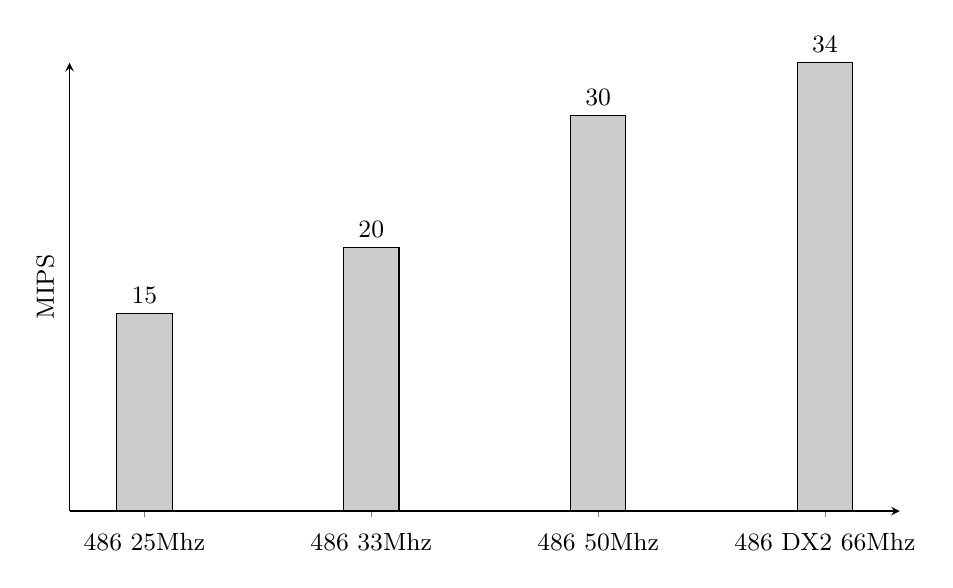
\begin{tikzpicture}[font=\small]
    \begin{axis}[
      width=1.0\textwidth,
      height=0.6\textwidth,
      ybar,
      bar width=20pt,
      ylabel={MIPS},
      ymin=0,
      ytick=\empty,
      xtick=data,
      axis x line=bottom,
      axis y line=left,
      enlarge x limits=0.11,
      symbolic x coords={486 25Mhz,486 33Mhz,486 50Mhz,486 DX2 66Mhz},
      xticklabel style={anchor=base,yshift=-\baselineskip},
      nodes near coords={\pgfmathprintnumber\pgfplotspointmeta}
    ]
      \addplot[fill=black!20,draw=black] coordinates {
        (486 25Mhz,15)
        (486 33Mhz,20)
        (486 50Mhz,30)
        (486 DX2 66Mhz,34)
      };
    \end{axis}
   
   \end{tikzpicture}
   \caption{Comparison\protect\footnotemark of CPUs with MIPS \protect\footnotemark.}
 \end{figure}
\footnotetext{Source: "Roy Longbottom's PC Benchmark Collection: http://www.roylongbottom.org.uk/mips.htm".}
\par
On the chart above, notice how a 486DX2-66Mhz is faster than a 485DX-50Mhz but not the full 20\% frequency could have made us expect. This is because the DX2 bus runs at 33Mhz while on the DX both CPU and the bus run at 50Mhz.




\subsection{Die}
%To close this section on the 486, I cannot resist including a magnified photography of the die. 
If you are holding a physical 9.25''x7.5'' copy of this book, the CPU packaging is 30mm square and the die is 15.5 x 9.9 mm, both represented at 1:1 scale.\\
\par
\bigskip

  \begin{figure}[!htb]

\begin{minipage}{0.48\textwidth}
\centering
\scaledrawimage{44.45mm}{486topdown.png}
%\caption{468 packaging.}
\end{minipage}
\hfill
\begin{minipage}{0.48\textwidth}
\centering
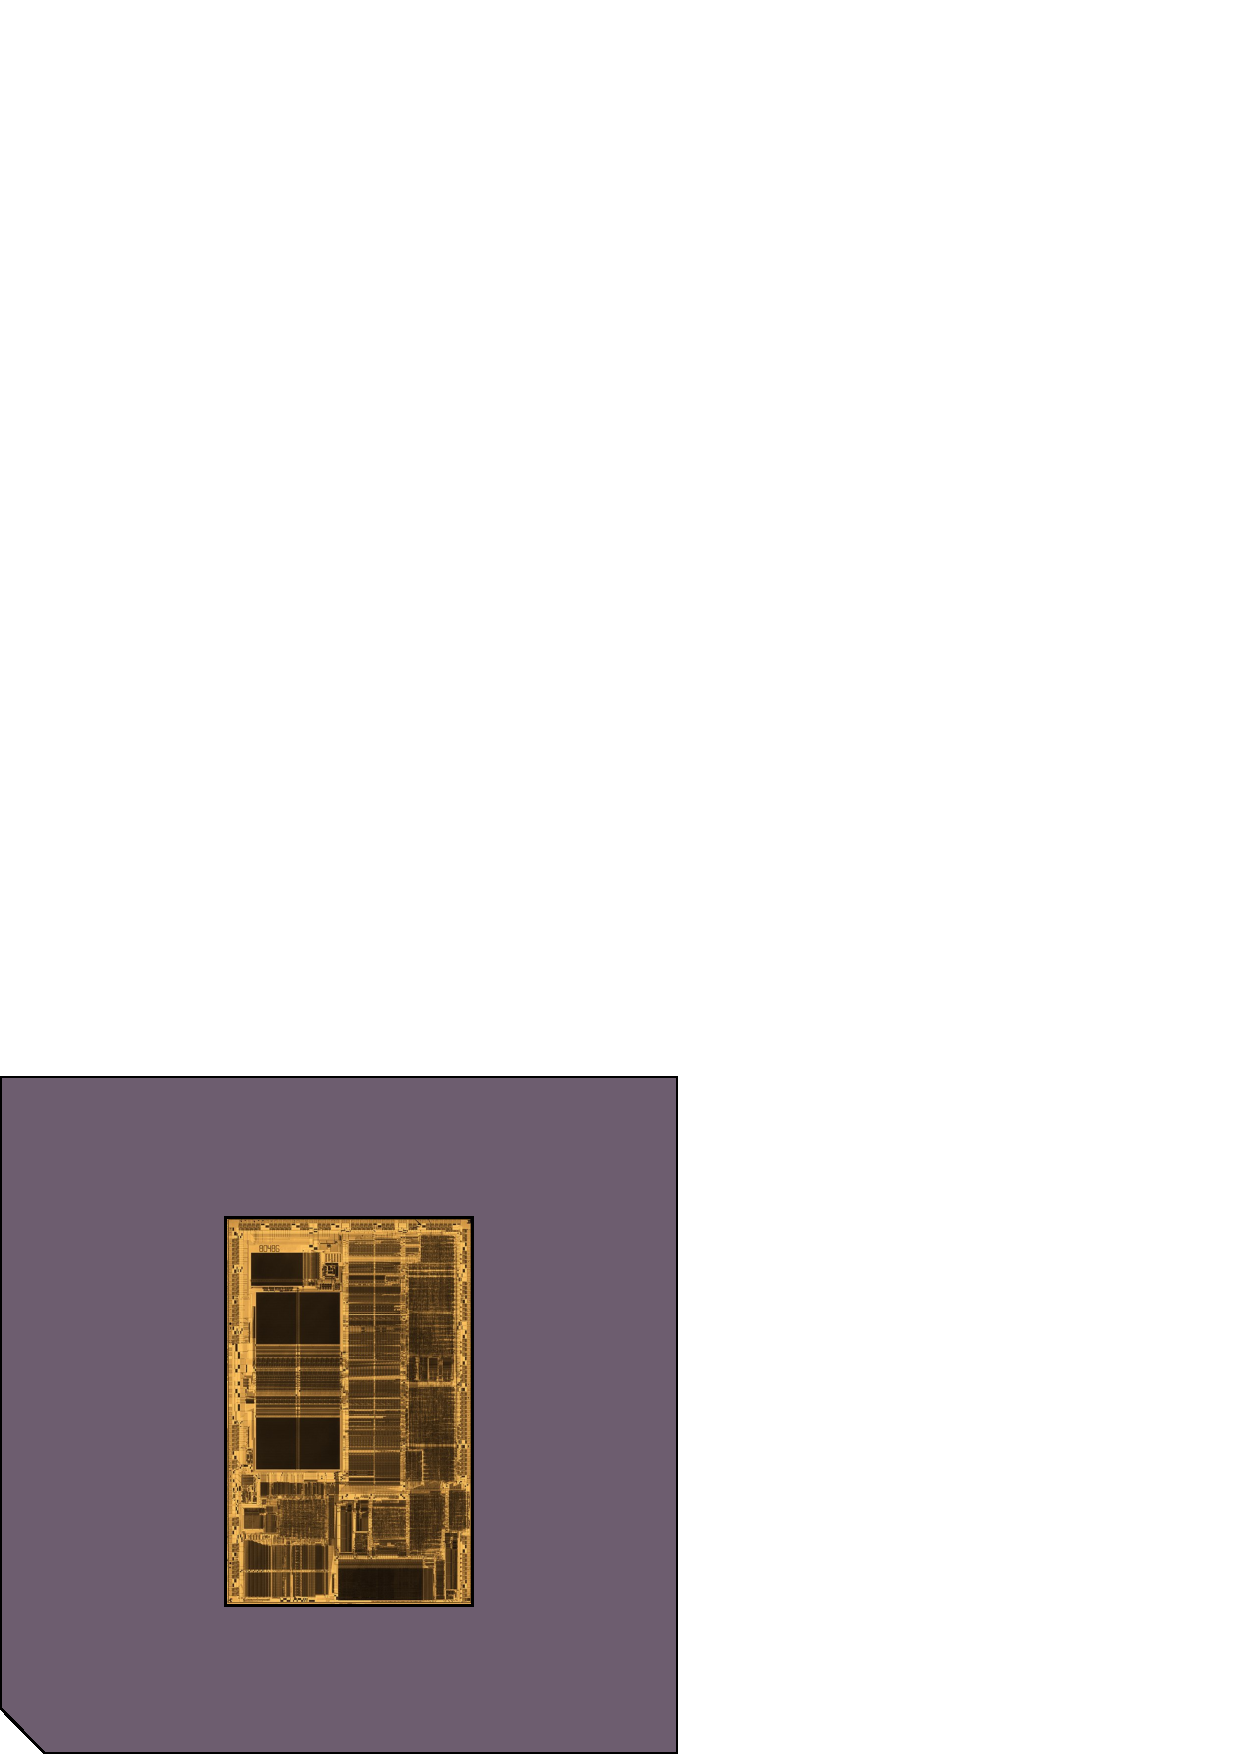
\includegraphics[width=44.45mm]{drawings/486toscale.pdf}
%\caption{The die inside the package.}
\end{minipage}
\end{figure}

\par



\begin{figure}[H]
\centering
\scaledimage{0.9}{486_blueprint.png}
\end{figure}
\par
\begin{figure}[H]
\centering
\scaledimage{0.9}{486_layout.png}
\end{figure}





On the previous page, the transistor layout differs between the data path which was hand-crafted and the control path which was created with CAD tools built especially for the 486\footnote{Source: Coping with the Complexity of Microprocessor
Design at Intel -- A CAD History.}.\\
\par
\subsection{Programming the 486}
With the architecture in mind we can now understand how a programmer could take best advantage of the 486. The good news was that most of the performance improvement was the characterized free-lunch of the 90s. The exact same binary would run twice as fast on the new CPU.\\
\par
Albeit a few peculiarities\footnote{"Pushing the 486" by Michael Abrash.}, as long as the programmer was mindful of the cacheline and maximized time and space locality\footnote{And avoid branching. Without a branch predictor, \cw{jmp} are ignored and usually incur a two cycles stale.}, the CPU would fly to process integers. Floating point operations had improved by a factor 2 compared to the i386's FPU (i387). In fact, floating point operations had improved so much that the i487 FPU could \cw{FMUL} faster than the i386 could \cw{IMUL}.\\
\par
\begin{figure}[H]
\centering
\begin{tabularx}{\textwidth}{ X  X X  X  X}
  \toprule
  \textbf{CPU} & \textbf{FADD} & \textbf{FMUL} & \textbf{FDIV} &\textbf{FXCH} \\ \bottomrule
Intel 387 & 23-34 & 29-57   & 88-91 & 18 \\
Intel 487 & 8-20  & 16   & 73 & 4 \\ \bottomrule
\end{tabularx}
\caption{FPU performance: 387 vs 487.}

\end{figure}

\par
But the FPU performance was still a far cry compared to the the ALU and its barrel shifter. This mandated \doom{} to use integer operations exclusively\footnote{The dawn of floating points would begin with Intel's Pentium and Quake in 1996.}.\\

\par
 \begin{figure}[H]
\centering  
\begin{tabularx}{\textwidth}{ L{0.3} L{0.3} L{0.4}}
  \toprule
  \textbf{Operation} &  \textbf{i486 (ALU)} & \textbf{i487 (FPU)} \\
  \toprule 
   
   \cw{ADD} & 1 & 8-20\\
   \cw{DIV} & 43 & 73\\
   \cw{MUL} & 12-42 & 29-52\\
   \toprule
\end{tabularx}
\caption{Comparaison ALU vs FPU operations.}
\end{figure}
\par
\trivia{Difficulty to access information birthed myths about \doom{} and floating point units. One endless thread which occurred on \cw{alt.games.doom} in 1994 helps to appreciate the state of things. The topic "Does a 486DX run Doom faster than an SX?" from July 1994 and its (filtered) five answers shows how difficult it was to reach the truth.}


\fq{\cw{My friend is buying a computer and doesn't see much reason to buy
a DX.  Any opinions?  (or hard facts :) ?).}}{\cw{Dave Gates@bestsd.sdsu.edu - 23 Jul 1994 05:28}}


\vspace{1mm}

\fq{\cw{DOOM runs *MUCH* faster on a 486DX/33 than on a 486SX/33.  Believe me,
I've seen it running on the 2 different machines in the same room.} }{\cw{BillyBoB 4@aol.com - 23 Jul 1994 10:45}}

\vspace{1mm}

\fq{\cw{They are *NOT* any different as far as CPU speed go.  Period.
The reason one (DX) is faster must have something to do with
probably the SX has an ISA video card, or no cache, or less
memory. Doom does NOT NOT NOT NOT use an FPU (math co-processor) so there will be no slowdown for the SX.}}{\cw{Chad Anson@daisy.cc.utexas.edu - 23 Jul 1994 11:48}}

\vspace{1mm}

\fq{\cw{We have a 486SX/25 and a 486DX/50 and the DX 50 runs faster at full screen
high detail then the SX runs at postage stamp. It is so slow as to be
almost unplayable.} }{\cw{BonesBro@aol.com - 23 Jul 1994 12:36}}

\vspace{1mm}

\fq{\cw{An SX is considerably slower than a DX for most processor-intensive
applications and games, including DOOM.}}{\cw{Neal W.Miller@@rebecca.its.rpi.edu - 23 Jul 1994 13:34}}

\vspace{1mm}

\fq{\cw{Thats wrong !
A 486 SX runs Doom with exactly the same speed like a 486 DX
(if you use the same VGA Card and Motherboard).}}{\cw{Grassl Wolfgang@papin.HRZ.Uni-Marburg.DE - 23 Jul 1994 14:24}}







